\documentclass{article}

\usepackage{exercises}
\withsolutions

\begin{document}
\sheet{NP-Vollständigkeit \& dynamische Programmierung}
\begin{exercise}{Independent Set}
  Ein Independent Set in einem Graphen $G = (V, E)$ ist eine Menge von Knoten $I$, so dass für je zwei Knoten $i, j \in I$ gilt, dass $(i, j) \notin E$. Für das Problem INDEPENDENT SET ist ein Graph $G = (V, E)$ sowie eine Zahl $k \in \mathbb{N}$ gegeben und es soll entschieden werden, ob es in $G$ ein Independent Set mit $k$ Knoten gibt.\par
  Zeigen Sie, dass das Problem INDEPENDENT SET NP-vollständig ist, indem Sie eine Reduktion von CLIQUE auf INDEPENDENT SET angeben.

  \begin{solution}
    \begin{itemize}
      \item Zunächst wollen wir zeigen, dass INDEPENDENT SET in NP liegt. Hierzu finden wir einen Algorithmus, welcher eine gegebene Lösung (Zertifikat) $I$ in polynomieller Zeit verifiziert:
            \begin{enumerate}
              \item Überprüfe, ob $I$ eine Menge von $k$ Knoten ist.
              \item Überprüfe, ob für je zwei Knoten $i, j \in I$ gilt, dass $(i, j) \notin E$.
            \end{enumerate}
      \item Nun wollen wir zeigen, dass CLIQUE $\leq_p$ INDEPENDENT SET. Eine Reduktionsfunktion könnte folgendermaßen aussehen:
            \begin{enumerate}
              \item Sei $G = (V, E)$ ein Graph und $k \in \mathbb{N}$.
              \item Erzeuge einen neuen Graphen $G' = (V, E')$ mit $E' = \{(i, j) \mid i, j \in V \land (i, j) \notin E\}$.
              \item Gebe die Eingabe $(G', k)$ zurück.
            \end{enumerate}
            Da ein Independent Set in $G'$ genau dann eine Clique in $G$ ist, ist die Reduktion korrekt. CLIQUE lässt sich somit auf INDEPENDENT SET reduzieren mit der Eingabe $(G, k) \mapsto (G', k)$.\par Somit ist INDEPENDENT SET NP-vollständig.
    \end{itemize}
  \end{solution}
\end{exercise}

\begin{exercise}{Textumbruch}
  Gegeben seien Wörter $w_1, \ldots, w_n$. Diese Wörter sollen auf Textzeilen aufgeteilt werden. Dazu seien $c(i, j)$ die Kosten, um Wörter die $w_i, \ldots, w_j$ in eine Textzeile zu schreiben für alle $1 \leq i \leq j \leq n$.\par
  Geben Sie mithilfe dynamischer Programmierung einen Algorithmus an, der Linebreaks $l_1, \ldots, l_m$ so setzt, sodass $c(1,l_1)+c(l_1 +1,l_2)+\ldots+c(l_m +1,n)$ minimiert wird.

  \begin{solution}
    \begin{itemize}
      \item \textbf{optimale Teilstruktur}: Wenn wir annehmen, dass die Gesamtkosten minimal sind, dann sind die Kosten für die Wörter $w_i, \ldots, w_j$ in einer Zeile minimal. Ansonsten könnten wir die Wörter in zwei Zeilen aufteilen und die Kosten wären kleiner. Außerdem ist die Aufteilung der Wörter in Zeilen unabhängig von der Aufteilung in anderen Zeilen. Somit ist die optimale Teilstruktur gegeben.
      \item \textbf{Rekursionsvorschrift}: Sei $D[i]$ die minimalen Kosten, um die Wörter $w_1, \ldots, w_i$ in Zeilen zu schreiben. Dann gilt \[
              D[j] = \begin{cases}
                c(1,j)                                & \text{falls } j=1 \\
                \min_{1\leq k\leq j}\{D[k-1]+c(k,j)\} & \text{falls } j>1
              \end{cases}
            \]
      \item \textbf{Algorithmus}: Ein Algorithmus in Pseudocode könnte wie folgt aussehen:\par\begin{algorithm}[H]
  \caption{\texttt{linebreaks($n, c$)}}\label{alg:linebreaks}

  \KwData{Anzahl der Wörter $n$ und Kostenfunktion $c$}
  \KwResult{Eine optimale Auswahl von Zeilenumbrüchen $breaks$ und die Kosten dieser Auswahl $costs[n]$}
  \BlankLine

  $costs \gets \emptyset$\;
  $breaks \gets \emptyset$\explain*{Speichert den letzten Zeilenumbruch vor Wort $i$}

  $costs[1] \gets c(1, 1)$\;
  \For{$j \gets 2$ \KwTo $n$}{
    $costs[j] \gets \infty$\;
    $breaks[j] \gets 0$\;
    \For{$k \gets 1$ \KwTo $j$}{
      $t \gets costs[k - 1] +  c(k, j)$\;
      \If{$t < costs[j]$}{
        $costs[j] \gets t$\;
        $breaks[j] \gets k$\;
      }
    }
  }

  \comment{Rekonstruktion der optimalen Lösung}
  $l \gets \emptyset$\explain*{Optimale Auswahl von Zeilenumbrüchen}
  $j \gets n$\;
  \While{$breaks[j] > 0$}{
    $l \gets \{breaks[j]\} \cup l$\;
    $j \gets breaks[j] - 1$\;
  }

  \Return $l, costs[n]$
\end{algorithm}
    \end{itemize}
  \end{solution}
\end{exercise}

\begin{eexercises}{Kursauswahl}{
    Stellen Sie sich vor Sie arbeiten in einer Behörde und haben ein bestimmtes Budget $B \in \mathbb{N}$, welches Sie ausgeben müssen. Dabei ist ein Kursangebot $K_1, \ldots, K_n$ gegeben wobei jeder Kurs $K_i$ gewisse Kosten $C_i \in \mathbb{N}$ hat und einen gewissen Organisationsaufwand $A_i \in \mathbb{N}$ benötigt. Gesucht ist eine Auswahl von Kursen, so dass mindestens das Budget $B$ ausgegeben wird und der gesamte Organisationsaufwand minimal ist.
  }
  \item Überlegen Sie sich einen einfachen Algorithmus, der eine Auswahl findet, die das Budget erfüllt (wenn eine existiert) und erläutern Sie kurz die Idee des Algorithmus. Der Algorithmus muss keine optimale Lösung finden und es muss kein Pseudocode angegeben werden.
  \item Geben Sie sich die Rekursionsvorschrift für ein dynamisches Programm für das Problem an und eine kurze Begründung für die Korrektheit der Formel. Verwenden Sie dafür eine Tabelle $D$, wobei $D[i, b]$ den minimalen Organisationsaufwand beinhalten soll um mit den Kursen $K_1, \ldots, K_i+1$ genau das Budget $b$ auszugeben.
  \item Geben Sie einen Algorithmus in Pseudocode basierend auf der Rekursionsvorschrift an, der eine optimale Auswahl findet.
\end{eexercises}

\begin{solutions}
  \item Ein einfacher Algorithmus könnte wie folgt aussehen:
  \begin{enumerate}
    \item Sortiere die Kurse aufsteigend nach dem Aufwand.
    \item Füge solange einen weiteren Kurs hinzu, bis das Budget erfüllt ist.
  \end{enumerate}
  \item Die Rekursionsvorschrift für das dynamische Programm ist\[
    D[i, b] = \begin{cases}
      0                                  & \text{falls } i=0 \land b=0 \\
      \infty                             & \text{falls } i=0 \land b>0 \\
      \min(D[i-1, b], D[i-1, b-C_i]+A_i) & \text{sonst}
    \end{cases}
  \] Der minimale Organisationaufwand entspricht entweder dem vorigen minimalen Aufwand oder dem minimalen Aufwand, der mit dem aktuellen Kurs erzielt werden kann. Falls das Budget nicht erfüllt wird, wird der Aufwand mit $\infty$ bestraft.
  \item Ein Algorithmus in Pseudocode könnte wie folgt aussehen:\par\begin{algorithm}[H]
  \caption{\texttt{pickCourses($n, B, C, A$)}}\label{alg:pickCourses}

  \KwData{Anzahl der Kurse $n$, Budget $B$, Kosten $C$, Organisationsaufwand $A$}
  \KwResult{Budgeterfüllende Kursauswahl $courses$ und minimaler Organisationsaufwand $D[n, B]$}
  \BlankLine

  $D \gets \text{Array of size } n \times B$\;
  \lFor{$i \gets 0$ \KwTo $n$}{$D[i, 0] \gets 0$}
  \lFor{$b \gets 0$ \KwTo $B$}{$D[0, b] \gets \infty$}

  \For{$i \gets 1$ \KwTo $n$}{
  \For{$b \gets 1$ \KwTo $B$}{
  $withoutCourse \gets D[i-1, b]$\;
  $withCourse \gets D[i-1, b-C[i]]+A[i]$\;

  \leIf{$withCourse < withoutCourse$}{
    $D[i, b] \gets withCourse$\;
  }{
    $D[i, b] \gets withoutCourse$
  }
  }
  }

  \comment{Rekonstruktion der optimalen Lösung}
  $courses \gets \emptyset$\;
  $b \gets B$\;
  \For{$i \gets n$ \KwTo $1$}{
  \If{$D[i, b] \neq D[i-1, b]$}{
  $courses \gets \{i\} \cup courses$\;
  $b \gets b-C[i]$\;
  }
  }

  \Return{$courses$, $D[n, B]$}
\end{algorithm}

\end{solutions}

\begin{eexercises}{Grundstückproblem}{
    Ein Grundstück soll mit möglichst großen Einnahmen verkauft werden. Das Grundstück ist rechteckig und liegt an einer Straße, welche durch ein Intervall $(0, S)$ repräsentiert wird. Es liegen $n$ Angebote mit Profiten $a_i$ für alle $i \in \{1, \ldots, n\}$ für Teile des Grundstücks vor. Diese Teile sind jeweils rechteckige Teilabschnitte mit Straßenzugang, die jeweils durch Teilintervalle $(l_i, r_i) \subseteq [0, S]$ repräsentiert sind. Das Ziel ist es nun eine Auswahl von Angeboten $A \subseteq \{1, \ldots, n\}$ zu finden, sodass die Angebote sich nicht überlappen – also $(l_i, r_i) \cap (l_j, r_j)=\emptyset$ für alle $i,j \in A$ mit $i \neq j$ – und der Profit $\sum_{i \in A} a_i$ möglichst groß ist.
    \hint{Es sei $z_1, \ldots, z_k$ eine aufsteigende Sortierung der Zahlen $\{0, S\} \cup \bigcup_{i=1}^n \{l_i, r_i\}$. Ein Ansatz für die Rekursionsformel wäre es nun für alle $j \in \{1, \ldots, k\}$, den maximalen Profit zu bestimmen, der mit Angeboten $i$ erzielt werden kann, für die $(l_i, r_i) \subseteq (0, z_j)$ gilt.}
    \begin{figure}
  \centering
  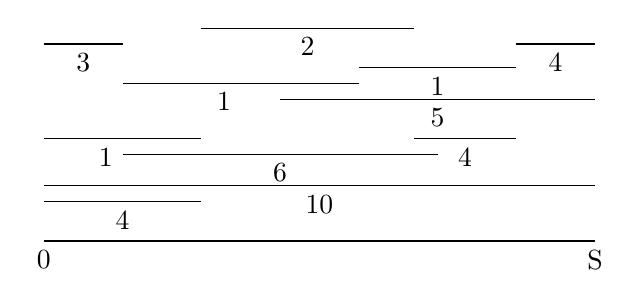
\begin{tikzpicture}
    \node at (0,0) [below] {0};
    \node at (7,0) [below] {S};

    \draw (2,2.7) -- node[below] {2} (4.7,2.7);
    \draw (0,2.5) -- node[below] {3} (1,2.5);
    \draw (6,2.5) -- node[below] {4} (7,2.5);
    \draw (4,2.2) -- node[below] {1} (6,2.2);
    \draw (1,2) -- node[below left] {1} (4,2);
    \draw (3,1.8) -- node[below] {5} (7,1.8);
    \draw (0,1.3) -- node[below left] {1} (2,1.3);
    \draw (4.7,1.3) -- node[below] {4} (6,1.3);
    \draw (1,1.1) -- node[below] {6} (5,1.1);
    \draw (0,.7) -- node[below] {10} (7,.7);
    \draw (0,.5) -- node[below] {4} (2,.5);
    \draw[thick] (0,0) -- (7,0);
  \end{tikzpicture}

  \caption{Ein Beispiel für das Grundstückproblem. Zahlen entsprechen den Profiten.}\label{fig:grundstueck}
\end{figure}
  }
  \item Finden Sie im gegebenen Beispiel (siehe \ref{fig:grundstueck}) eine optimale Auswahl.
  \item Geben Sie die Rekursionsvorschrift für ein dynamisches Programm für das Problem an und eine kurze Begründung für die Korrektheit der Formel.
  \item Beschreiben Sie kurz wie basierend auf der Formel ein Algorithmus für das Problem entworfen werden kann und schätzen Sie die entsprechende Laufzeit ab.
  \item Wieviel Zeit benötigt ein Brute-Force-Algorithmus, der alle Teilmengen $A \subseteq [n]$ überprüft?
\end{eexercises}

\begin{solutions}
  \item Im gegebenen Beispiel ist eine optimale Auswahl $\{4, 2, 4, 4\}$ mit einem Profit von $14$.
  \item Die Rekursionsvorschrift für das dynamische Programm ist \[
    P[j] = \begin{cases}
      0                                                                                          & \text{falls } j = 0                     \\
      \max(P[j-1], \max_{1\leq i\leq n\text{ und } (l_i,r_i) \subseteq (0,z_j)}\{P[l_i-1]+a_i\}) & \text{für alle } j \in \{1, \ldots, k\}
    \end{cases}
  \] Der maximale Profit entspricht entweder dem vorigen maximalen Profit oder dem maximalen Profit, der mit einem Angebot erzielt werden kann, dessen Teilintervall in $(0, z_j)$ liegt.
  \item Ein Algorithmus kann basierend auf der Rekursionsvorschrift wie folgt aussehen:
  \begin{enumerate}
    \item Sortiere die Zahlen $\{0, S\} \cup \bigcup_{i=1}^n \{l_i, r_i\}$ aufsteigend und entferne Duplikate.
    \item Initialisiere ein Array $P$ der Länge $k$ mit $0$.
    \item Iteriere über alle $j \in \{1, \ldots, k\}$ und setze $P[j]$ gemäß der Rekursionsvorschrift.
    \item Gehe rückwärts durch $P$ und bestimme die Auswahl von Angeboten, die den maximalen Profit erzielt.
  \end{enumerate}
  Die Laufzeit des Algorithmus beträgt $\mathcal{O}(n^2)$.
  \item Ein Brute-Force-Algorithmus benötigt $\mathcal{O}(2^n)$ Zeit. Denn es gibt $2^n$ Teilmengen von $[n]$, da es für jedes Element in $[n]$ zwei Möglichkeiten gibt: Es ist in der Auswahl oder nicht.
\end{solutions}

\begin{eexercises}{Entscheidungsproblem des Knapsack Problems}{
    Bei der Entscheidungsversion des Knapsack Problems sind Gewichte $w_1, \ldots, w_n \in \mathbb{N}$, Profite $p_1, \ldots, p_n \in \mathbb{N}$, ein Maximalgewicht $W \in \mathbb{N}$ und ein Mindestprofit $P \in \mathbb{N}$ gegeben. Es soll entschieden werden, ob eine Auswahl $M \subseteq \{1, \ldots, n\}$ existiert bei der beide Schranken eingehalten werden, also $\sum_{i \in M} p_i \geq P$ und $\sum_{i \in M} w_i \leq W$.
  }
  \item Zeigen Sie $\text{KNAPSACK} \in \text{NP}$.
  \item Zeigen Sie $\text{SUBSETSUM} \leq_p \text{KNAPSACK}$.
  \hint{Bei SUBSETSUM sind Zahlen $z_1, \ldots, z_n \in \mathbb{N}$ und ein Zielwert $T$ gegeben und es soll entschieden werden, ob eine Auswahl $S \subseteq \{1, \ldots, n\}$ existiert mit $\sum_{i \in S} z_i = T$.}
\end{eexercises}

\begin{solutions}
  \item Ein Algorithmus, der eine gegebene Lösung (Zertifikat) $M$ in polynomieller Zeit verifiziert, könnte wie folgt aussehen:
  \begin{enumerate}
    \item Überprüfe, ob $\sum_{i \in M} p_i \geq P$.
    \item Überprüfe, ob $\sum_{i \in M} w_i \leq W$.
  \end{enumerate}
  \item Eine Reduktion von SUBSETSUM auf KNAPSACK könnte wie folgt aussehen:
  \begin{enumerate}
    \item Seien Zahlen $z_1, \ldots, z_n \in \mathbb{N}$ und ein Zielwert $T$ gegeben.
    \item Setze $w_i = z_i$ und $p_i = z_i$ für alle $i \in \{1, \ldots, n\}$.
    \item Setze $W = T$ und $P = T$.
    \item Gebe die Eingabe $(w_1, \ldots, w_n, p_1, \ldots, p_n, W, P)$ zurück.
  \end{enumerate}
  Da eine Auswahl $S \subseteq \{1, \ldots, n\}$ existiert mit $\sum_{i \in S} z_i = T$ genau dann, wenn eine Auswahl $M \subseteq \{1, \ldots, n\}$ existiert bei der beide Schranken eingehalten werden, ist die Reduktion korrekt. SUBSETSUM lässt sich somit auf KNAPSACK reduzieren mit der Eingabe $(z_1, \ldots, z_n, T) \mapsto (w_1, \ldots, w_n, p_1, \ldots, p_n, W, P)$.
\end{solutions}

\begin{eexercises}{NAE-k-SAT}{
    Eine NAE-k-SAT (Not-All-Equal) Formel hat folgende Form $\bigwedge_{i=1}^m (z_1^i, \dots, z_k^i)$, wobei eine Klausel $(z_1^i, \dots, z_k^i)$ mit Literalen $z_1^i, \dots, z_k^i$ genau dann erfüllt ist, wenn mindestens ein Literal zu wahr und mindestens ein Literal zu falsch ausgewertet wird.
    \hint{ (Beispiel) Für die NAE-3-SAT Formel $(x, y, z) \land (\neg x, y, z)$ ist durch $x = y = z = \text{true}$ keine erfüllende Belegung gegeben, da in diesem Fall die erste Klausel nicht erfüllt ist. Bei der Belegung $x = y = \text{true}$ und $z = \text{false}$ hingegen ist die Formel erfüllt.}
  }
  \item Zeigen Sie, dass für jede erfüllende Belegung einer NAE-k-SAT, die invertierte Belegung (jede mit true belegte Variable wird mit false belegt und andersrum) ebenfalls eine erfüllende Belegung ist.
  \item Zeigen Sie NAE-k-SAT $\in \text{NP}$.
  \item Zeigen Sie $3\text{-SAT} \leq_p \text{NAE-4-SAT}$.
\end{eexercises}

\begin{solutions}
  \item Sei $z_1, \ldots, z_k$ eine erfüllende Belegung einer NAE-k-SAT. Dann gibt es mindestens ein Literal $z_i$ mit $z_i = \text{true}$ und mindestens ein Literal $z_j$ mit $z_j = \text{false}$. Die invertierte Belegung hat dann $z_i = \text{false}$ und $z_j = \text{true}$, also ebenfalls mindestens ein Literal $z_i$ mit $z_i = \text{true}$ und mindestens ein Literal $z_j$ mit $z_j = \text{false}$.
  \item Ein Algorithmus, der eine gegebene Lösung (Zertifikat) $z_1, \ldots, z_k$ in polynomieller Zeit verifiziert, könnte wie folgt aussehen:
  \begin{enumerate}
    \item Überprüfe, ob für jede Klausel $(z_1^i, \dots, z_k^i)$ mindestens ein Literal zu wahr und mindestens ein Literal zu falsch ausgewertet wird.
  \end{enumerate}
  \item Eine Reduktion von $3\text{-SAT}$ auf $\text{NAE-4-SAT}$ könnte wie folgt aussehen:
  \begin{enumerate}
    \item Sei eine $3\text{-SAT}$ Formel $\varphi = \bigwedge_{i=1}^m (z_1^i, z_2^i, z_3^i)$ gegeben.
    \item Erzeuge eine $\text{NAE-4-SAT}$ Formel $\varphi' = \bigwedge_{i=1}^m (z_1^i, z_2^i, z_3^i, z_4^i)$.
    \item Gebe die Eingabe $\varphi'$ zurück.
  \end{enumerate}
  Da eine $3\text{-SAT}$ Formel $\varphi$ genau dann erfüllt ist, wenn die entsprechende $\text{NAE-4-SAT}$ Formel $\varphi'$ erfüllt ist, ist die Reduktion korrekt. $3\text{-SAT}$ lässt sich somit auf $\text{NAE-4-SAT}$ reduzieren.
\end{solutions}

\begin{exercise}{Floyd-Warshall Algorithmus}
  \begin{figure}
  \centering
  \begin{tikzpicture}[->, auto, on grid, bend left=.5cm, node distance=4cm, main node/.style={circle, draw, minimum size=.5em}]
    \node[main node] (A) {A};
    \node[main node] (B) [left=of A] {B};
    \node[main node] (C) [below right=2cm and 2cm of B] {C};
    \node[main node] (D) [below of=B] {D};

    \path[every node]
    (A) edge node {6} (B) edge node {3} (C) edge [bend left=2cm] node {10} (D)
    (B) edge node {13} (A) edge node {-2} (C) edge node {7} (D)
    (C) edge node {5} (A) edge node {5} (B) edge node {10} (D)
    (D) edge [bend right=1.5cm] node {-7} (A) edge node {7} (B) edge node {5} (C)
    ;
  \end{tikzpicture}

  \caption{Graph zum Floyd-Warshall Algorithmus.}\label{fig:floydwarshall}
\end{figure}
  Wenden Sie auf den Graphen aus \ref{fig:floydwarshall} den Algorithmus von Floyd-Warshall an und geben Sie nach jeder Iteration der ersten Schleife die zugehörige Distanzmatrix an. Nehmen Sie an, dass Knoten zu sich selbst einen Abstand von 0 haben. Betrachten Sie die Knoten in der Reihenfolge A, B, C, D. Welches Knotenpaar besitzt den größten/kürzesten Abstand?
  \begin{solution}
    \begin{table}
      \centering
      \begin{tabular}{cccc}
        Iteration 0 & Iteration 1 & Iteration 2 & Iteration 3 \\
        $
          \begin{pmatrix}
            0 & 2 & 4 & 5 \\
            2 & 0 & 3 & 4 \\
            4 & 3 & 0 & 1 \\
            5 & 4 & 1 & 0
          \end{pmatrix}
        $           & $
          \begin{pmatrix}
            0 & 2 & 4 & 5 \\
            2 & 0 & 3 & 4 \\
            4 & 3 & 0 & 1 \\
            5 & 4 & 1 & 0
          \end{pmatrix}
        $           & $
          \begin{pmatrix}
            0 & 2 & 4 & 5 \\
            2 & 0 & 3 & 4 \\
            4 & 3 & 0 & 1 \\
            5 & 4 & 1 & 0
          \end{pmatrix}
        $           & $
          \begin{pmatrix}
            0 & 2 & 4 & 5 \\
            2 & 0 & 3 & 4 \\
            4 & 3 & 0 & 1 \\
            5 & 4 & 1 & 0
          \end{pmatrix}
        $
      \end{tabular}
    \end{table}
    Das Knotenpaar mit dem größten Abstand ist $(A, D)$ mit einem Abstand von 4. Das Knotenpaar mit dem kürzesten Abstand ist $(A, B)$ mit einem Abstand von 2.
  \end{solution}
\end{exercise}
\end{document}